\chapter[Steady-state full-core MSBR benchmark]{Steady-state full-core MSBR benchmark}

\section{SERPENT 2 code overview}
SERPENT is a continuous-energy Monte Carlo neutronics software capable of solving the neutron transport problem by tracking individual neutrons within the problem geometry and using stochastic method to determine chain of events for each neutron \cite{leppanen_serpent_2015}. SERPENT has been under active development at the VTT Technical Research Centre of Finland since 2004, where it was initially conceived as a tool to simplify group constant generation in a high-fidelity Monte Carlo environment. SERPENT is now widely used transport code  with a growing user base. Now SERPENT used by more than 500 registered individuals in 155 organizations located in 37 countries around the world. The burnup calculation capability in SERPENT is based on built-in calculation routines, without using any external solvers. A restart feature allows performing fuel shuffling or applying any modifications in the input by dividing the calculation into several parts, which is crucial for online reprocessing simulations.

The latest version, SERPENT 2, supports advanced geometries and has advanced burnup capabilities, including online refueling capabilities which are necessary for neutronic computations of pebble-bed reactors and liquid-fueled \glspl{MSR} \cite{aufiero_extended_2013}. Unfortunately, built-in online refueling features are still under active development and unavailable to ordinary users. Furthermore, recently multi-physics simulations using SERPENT 2 were demonstrated, i.e. coupled calculations with thermal-hydraulics, \gls{CFD} and fuel performance codes \cite{leppanen_numerical_2015}. Two-way coupling to thermal-hydraulics, \gls{CFD}, and fuel performance codes operates on two levels: internal coupling to built-in solvers for fuel behavior and thermal-hydraulics, and external coupling via a universal multi-physics interface. 

SERPENT 2 can be effectively run in parallel on computer clusters and multi-core workstations. Parallelization is handled by thread-based OpenMP, which has the advantage that all processsors use shared memory space. Calculations can be divided into several nodes by distributed-memory \gls{MPI} parallelization. SERPENT 2  is an improvement upon SERPENT 1, and contains a complete redesign of memory management using hybrid OpenMP \cite{dagum_openmp:_1998} + \gls{MPI} parallelization.  This hybrid parallelization is important in depletion calculations using computer clusters with multiple nodes, and allows to achieve significant speed-up in depletion calculations on computer clusters with more than 4'000 cores \cite{leppanen_serpent_2015-1}. 

All calculations presented in this thesis were performed using SERPENT 2 version 2.1.30 on Blue Waters’ XE6 nodes. For cross section generation, JEFF-3.1.2 nuclear data library was employed \cite{oecd/nea_data_bank_jeff-3.1.2_2014}. 

\section{Molten Salt Breeder Reactor description}
Figure~\ref{fig:ref_sect_msbr} shows the \gls{MSBR} vessel which has a diameter of 680 cm and a height of 610 cm. It contains a molten fluoride fuel-salt mixture that generates heat in the active core region and transports that heat to the primary heat exchanger by way of the primary salt pump. In the active core region, the salt flows through channels in moderating and reflecting graphite blocks. Salt at about 565$^{\circ}$C enters the central manifold at the bottom via four 40.64-cm-diameter nozzles and flows upward through channels in the lower plenum graphite. The fuel salt exits at the top at about 704$^{\circ}$C through four equally spaced nozzles which connect to the salt-suction pipes leading to primary circulation pumps. The fuel salt drain lines connect to the bottom of the reactor vessel inlet manifold.

Since reactor graphite experiences significant dimensional changes due to neutron irradiation, the reactor core was designed for periodic replacement. The reference \gls{MSBR} design has an average core power density of approximately 6.666 W/g. Based on the irradiation experimental data from \gls{MSRE}, core graphite lifetime density is about 4 years and reflector graphite lifetime is 30 years \cite{robertson_conceptual_1971}.

\begin{figure}[htp!] % replace 't' with 'b' to 
  \centering
  \vspace{-0.3em}
  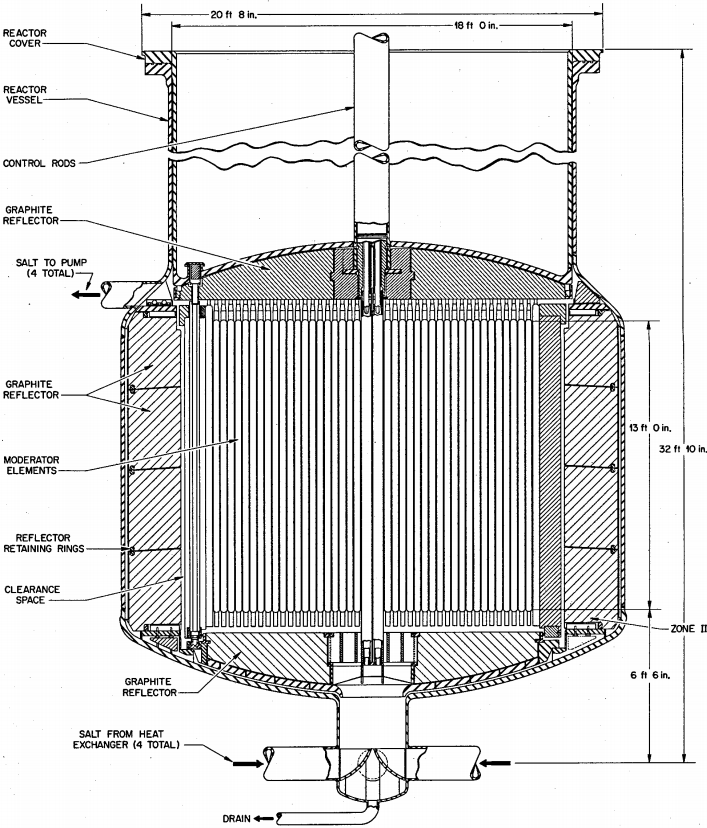
\includegraphics[width=\textwidth]{elev_view_vessel.png}
  \caption{Sectional elevation of \gls{MSBR} vessel \cite{robertson_conceptual_1971}.}
  \vspace{-0.6em}
  \label{fig:ref_sect_msbr}
\end{figure}

Moreover, it was decided to remove and install the core graphite as an assembly rather than by individual blocks, because it is relatively easier for maintenance personnel and has lower probability of radioactive elements escape due to used blocks damage during removal. In addition, handling the core as an assembly also allows the replacement core to be carefully preassembled and tested under factory conditions.

Figure~\ref{fig:ref_sect_msbr} and \ref{fig:ref_plan_msbr} demonstrate the configuration of the \gls{MSBR} vessel, core configuration, ``fission" (zone I) and ``breeding" (zone II) regions inside the vessel. The core has two radial zones bounded by a solid cylindrical graphite reflector and the vessel wall. The central zone, zone I, in which 13\% of the volume is fuel salt and 87\% graphite. Zone I composed of 1,320 graphite cells, 2 graphite control rods, and 2 safety\footnote{These rods needed for emergency shutdown only.} rods. The under-moderated zone, zone II, with 37\% fuel salt, and radial reflector, surrounds the zone I core region and serves to diminish neutron leakage. Zones I and II are surrounded radially and axially by fuel salt. This space for fuel is necessary for injection and flow of molten salt.

\begin{figure}[hbp!] % replace 't' with 'b' to 
  \centering
  \vspace{-0.3em}
  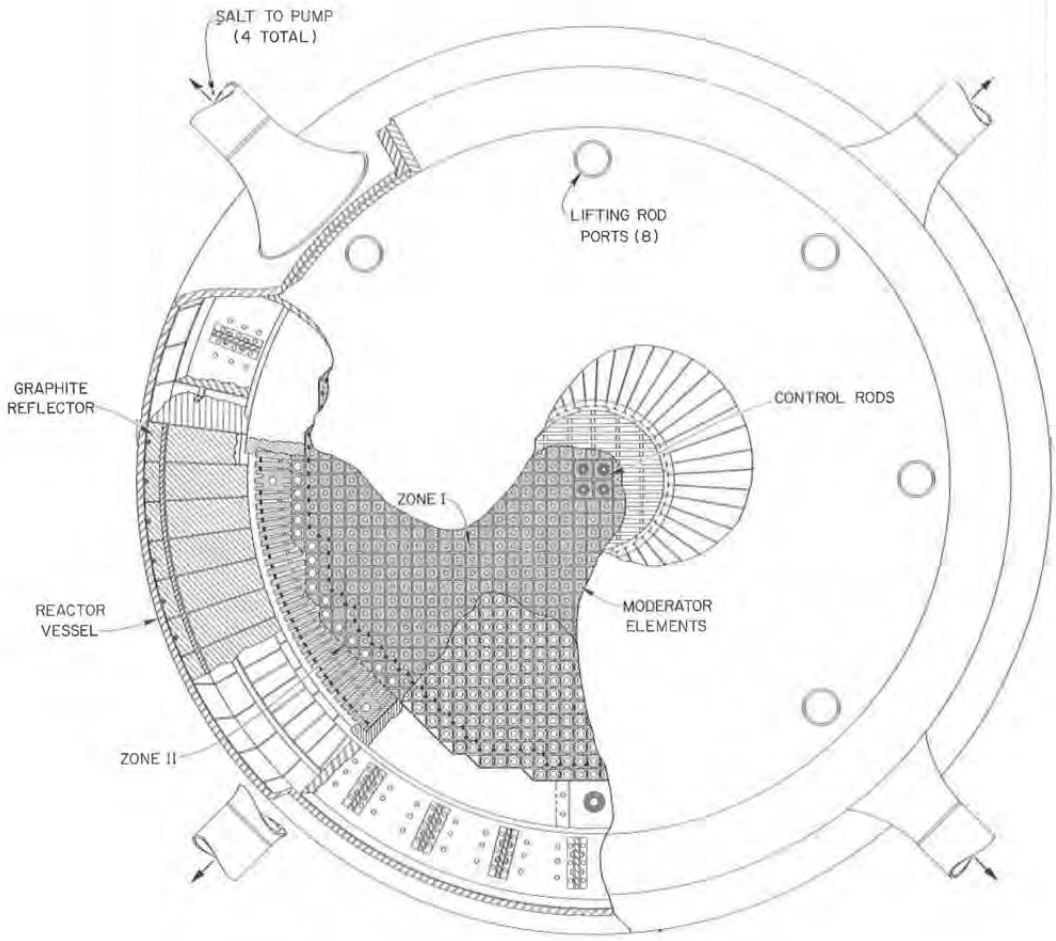
\includegraphics[width=\textwidth]{plan_view_vessel.png}
  \caption{Plan view of \gls{MSBR} vessel \cite{robertson_conceptual_1971}.}
  \vspace{-0.6em}
  \label{fig:ref_plan_msbr}
\end{figure}
\FloatBarrier

There are eight symmetric graphite slabs with a width of 15.24 cm in zone II, one of which is illustrated in Fig.~\ref{fig:detail_plan_view}. The holes in the centers are for the core lifting rods used during the core replacement operations. These holes also allow a portion of the fuel salt to flow to the top of the vessel for cooling the top head and axial reflector. Fig.~\ref{fig:detail_plan_view} also demonstrates the 5.08-cm-wide annular space between the removable core graphite in zone II-B and the permanently mounted reflector graphite. This annulus constists entirely of fuel salt, provides space for moving the core assembly, helps compensate the elliptical dimensions of the reactor vessel, and serves to reduce the damaging flux at the surface of the graphite reflector blocks.

\begin{figure}[hbp!] % replace 't' with 'b' to 
  \centering
  \vspace{-0.3em}
  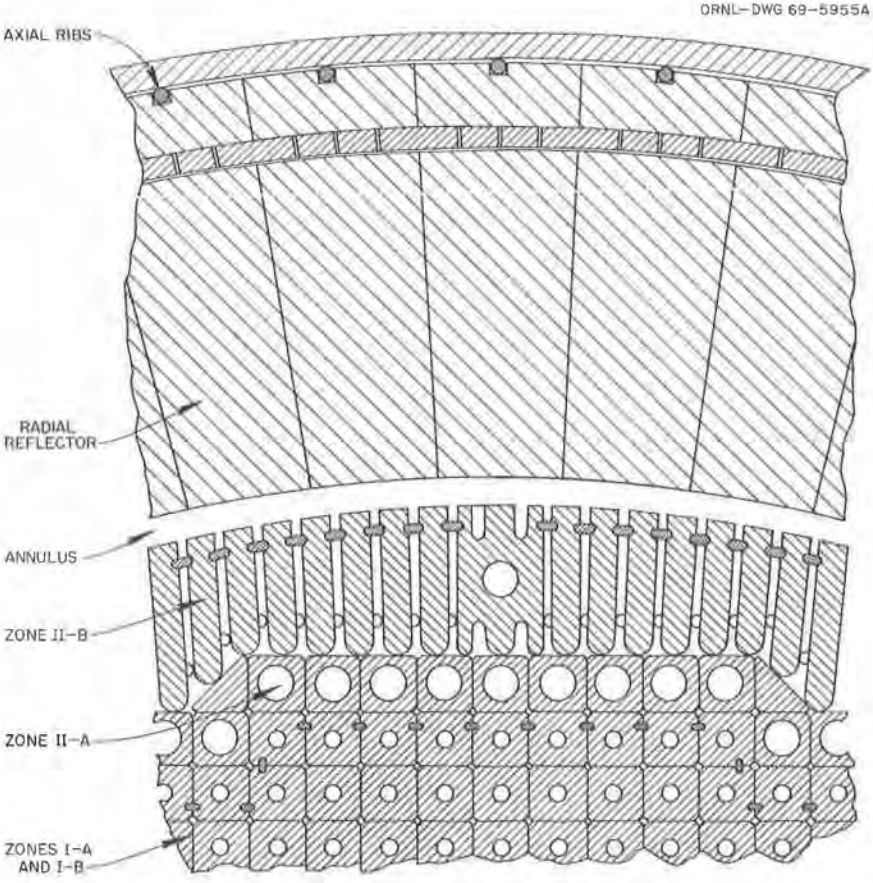
\includegraphics[width=\textwidth]{reflector_elements_ref.png}
  \caption{Detailed plan view of graphite reflector and moderator elements \cite{robertson_conceptual_1971}.}
  \vspace{-0.6em}
  \label{fig:detail_plan_view}
\end{figure}
\FloatBarrier

\subsection{Core zone I}
The central region of the core, called zone I, is made up of graphite elements, each $10.16$cm$\times$10.16cm$\times$396.24cm. In zone I, 13\% of the volume is fuel salt and 87\% is graphite. Zone I is composed of 1,320 graphite cells and 4 channels for control rods: two for graphite rods which both regulate and shim during normal operation, and two for backup safety rods consisting of boron carbide clad to assure sufficient negative reactivity for emergency situations.

These graphite elements have a mostly rectangular shape with lengthwise ridges at each corner that leave space for salt flow elements. Various element sizes reduce the peak damage flux and power density in the center of the core to prevent local graphite damage. Zone I is well-moderated to achieve the desired fission power density. Figure~\ref{fig:I_element_ref} demonstrates the elevation and sectional views of graphite elements of zone I \cite{robertson_conceptual_1971} and their SERPENT model \cite{rykhlevskii_full-core_2017}.

\subsection{Core zone II}
Zone II which is undermoderated, surrounds zone I. Combined with the bounding radial reflector, zone II serves to diminish neutron leakage. This zone is formed of two kinds of elements: large-diameter fuel channels (zone II-A) and radial graphite slats (zone II-B). 

Zone II has 37\% fuel salt by volume and each element has a fuel channel diameter of 6.604cm. The graphite elements for zone II-A are prismatic and have elliptical-shaped dowels running axially between the prisms and needed to isolate the fuel salt flow in zone I from that in zone II. Fig.~\ref{fig:II_element_ref} shows shape and dimensions of these graphite elements and their SERPENT model. Zone II-B elements are rectangular slats spaced far enough apart to provide the 0.37 fuel salt volume fraction. The reactor zone II-B graphite 5.08cm-thick slats vary in the radial dimension (average width is 26.67cm) as shown in figure~\ref{fig:detail_plan_view}. Zone II serves as a blanket to achieve the best performance: a high breeding ratio and a low fissile inventory. The neutron energy spectrum in zone II is made harder to enhance the rate of thorium resonance capture relative to the fission rate, thus limiting the neutron flux in the outer core zone and reducing the neutron leakage \cite{robertson_conceptual_1971}. 

\begin{figure}[hbp!] % replace 't' with 'b' to 
  \centering
  \vspace{-0.3em}
  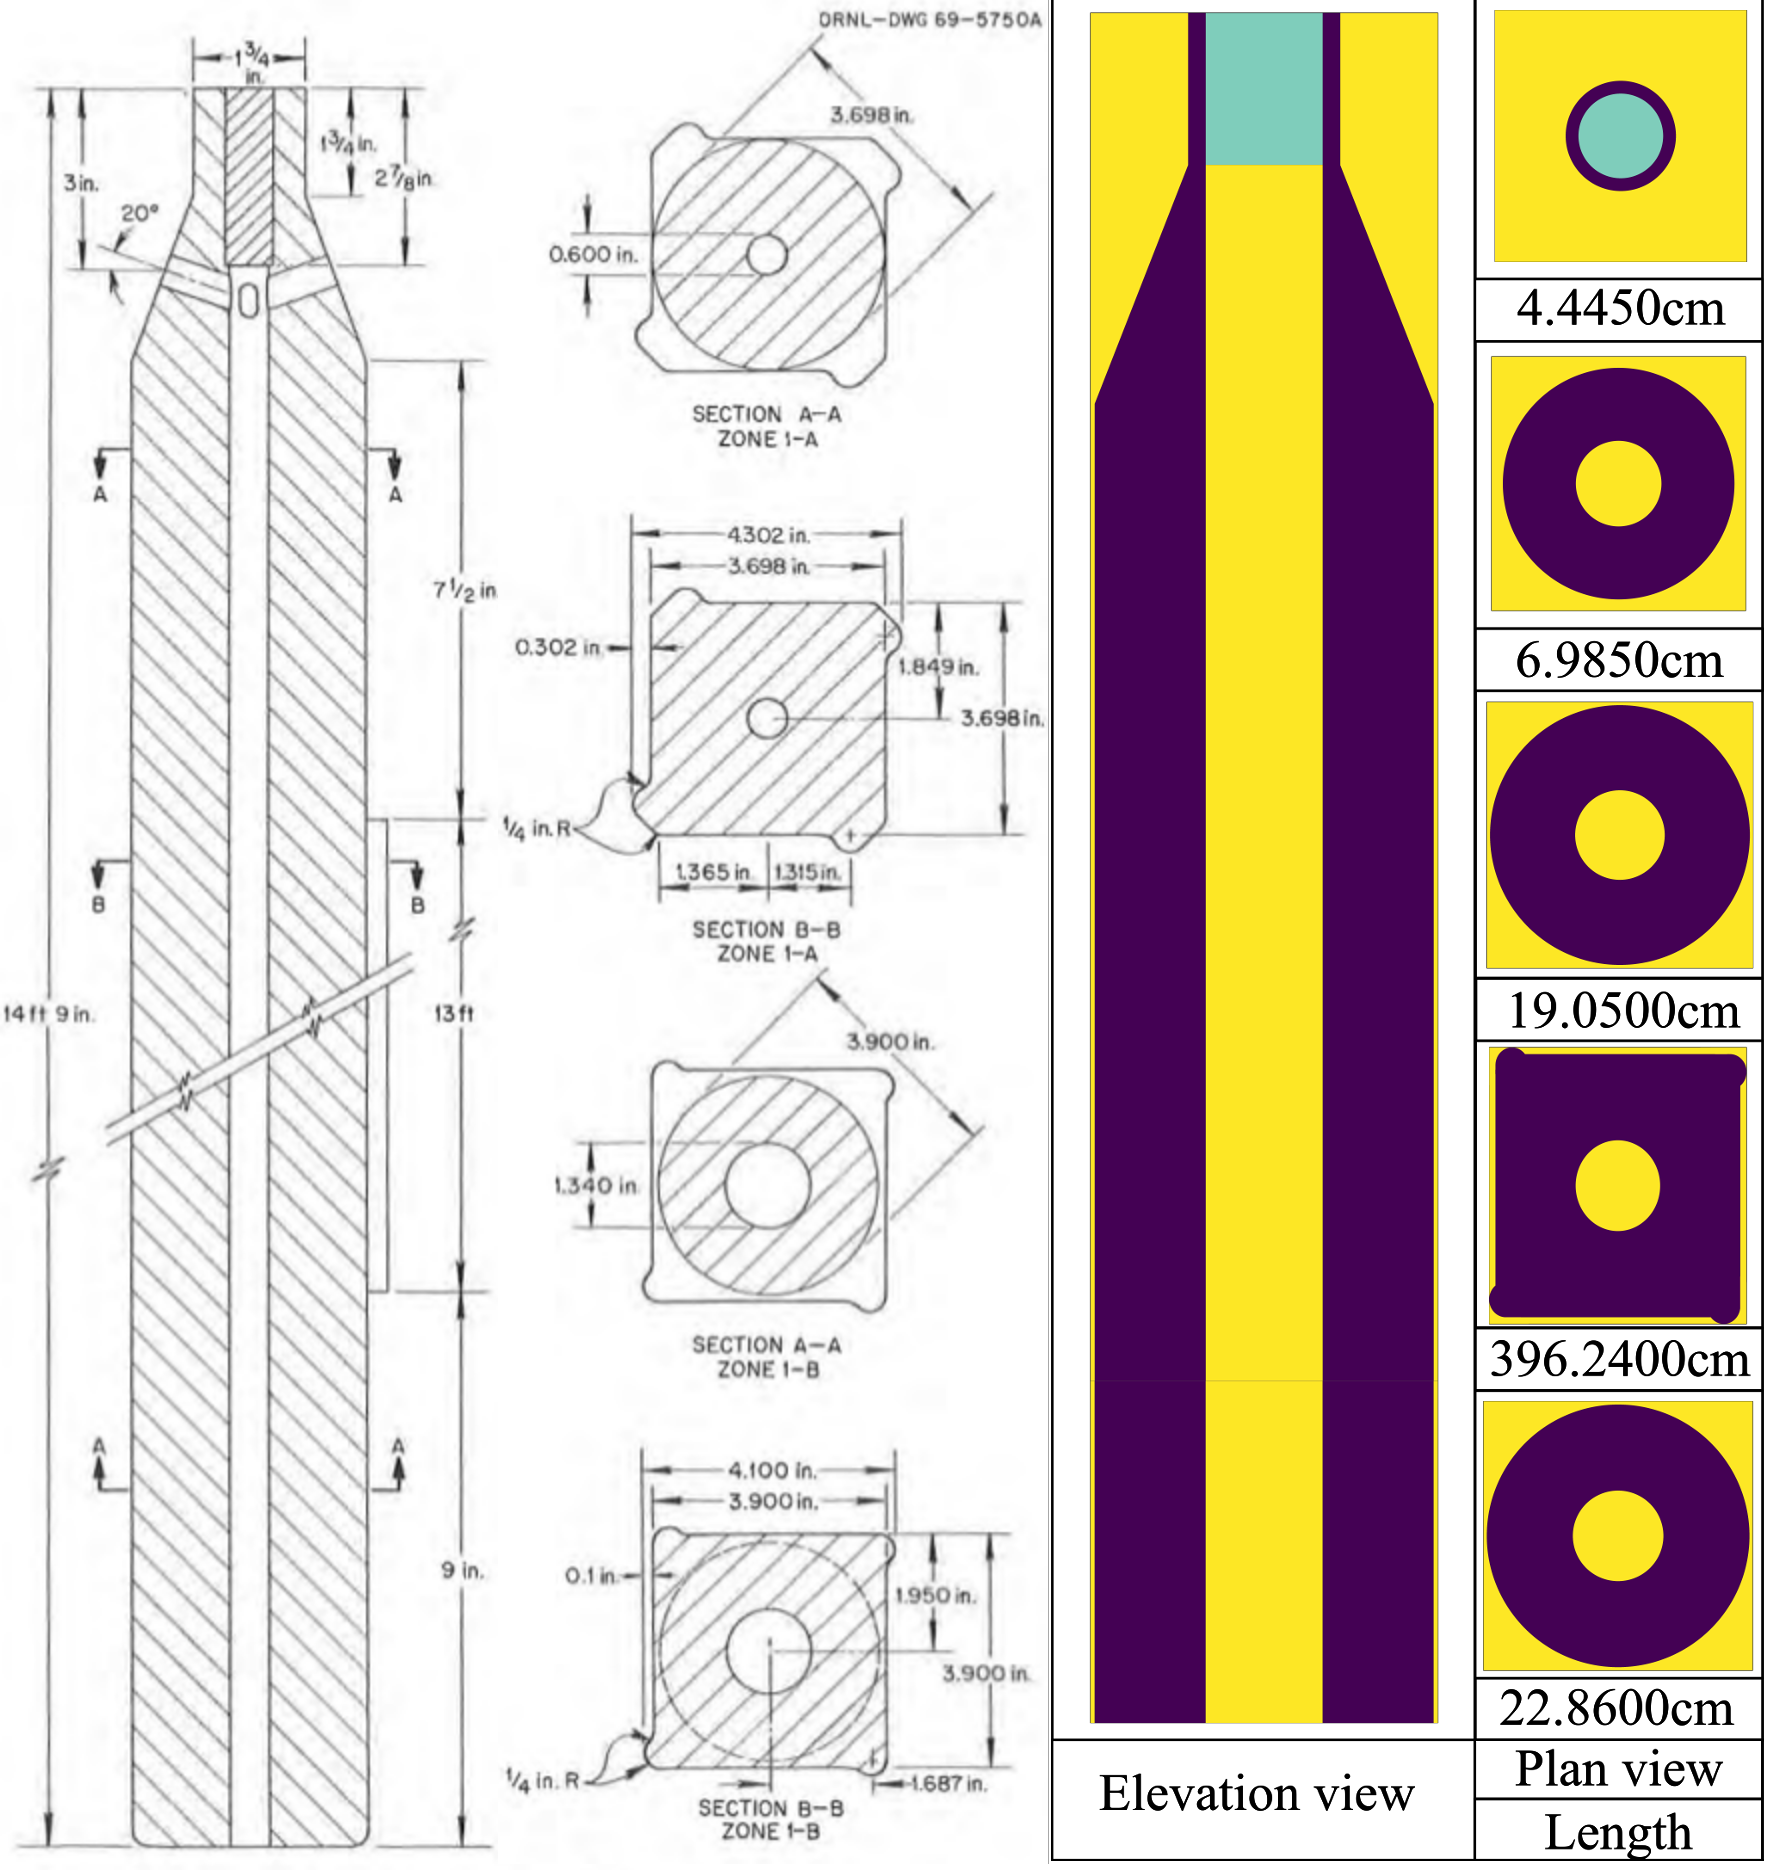
\includegraphics[width=\textwidth]{zone_I_element_ref.png}
  \caption{Graphite moderator elements for zone I \cite{robertson_conceptual_1971,rykhlevskii_full-core_2017}.}
  \vspace{-0.6em}
  \label{fig:I_element_ref}
\end{figure}
\FloatBarrier

\begin{figure}[hbp!] % replace 't' with 'b' to 
  \centering
  \vspace{-0.3em}
  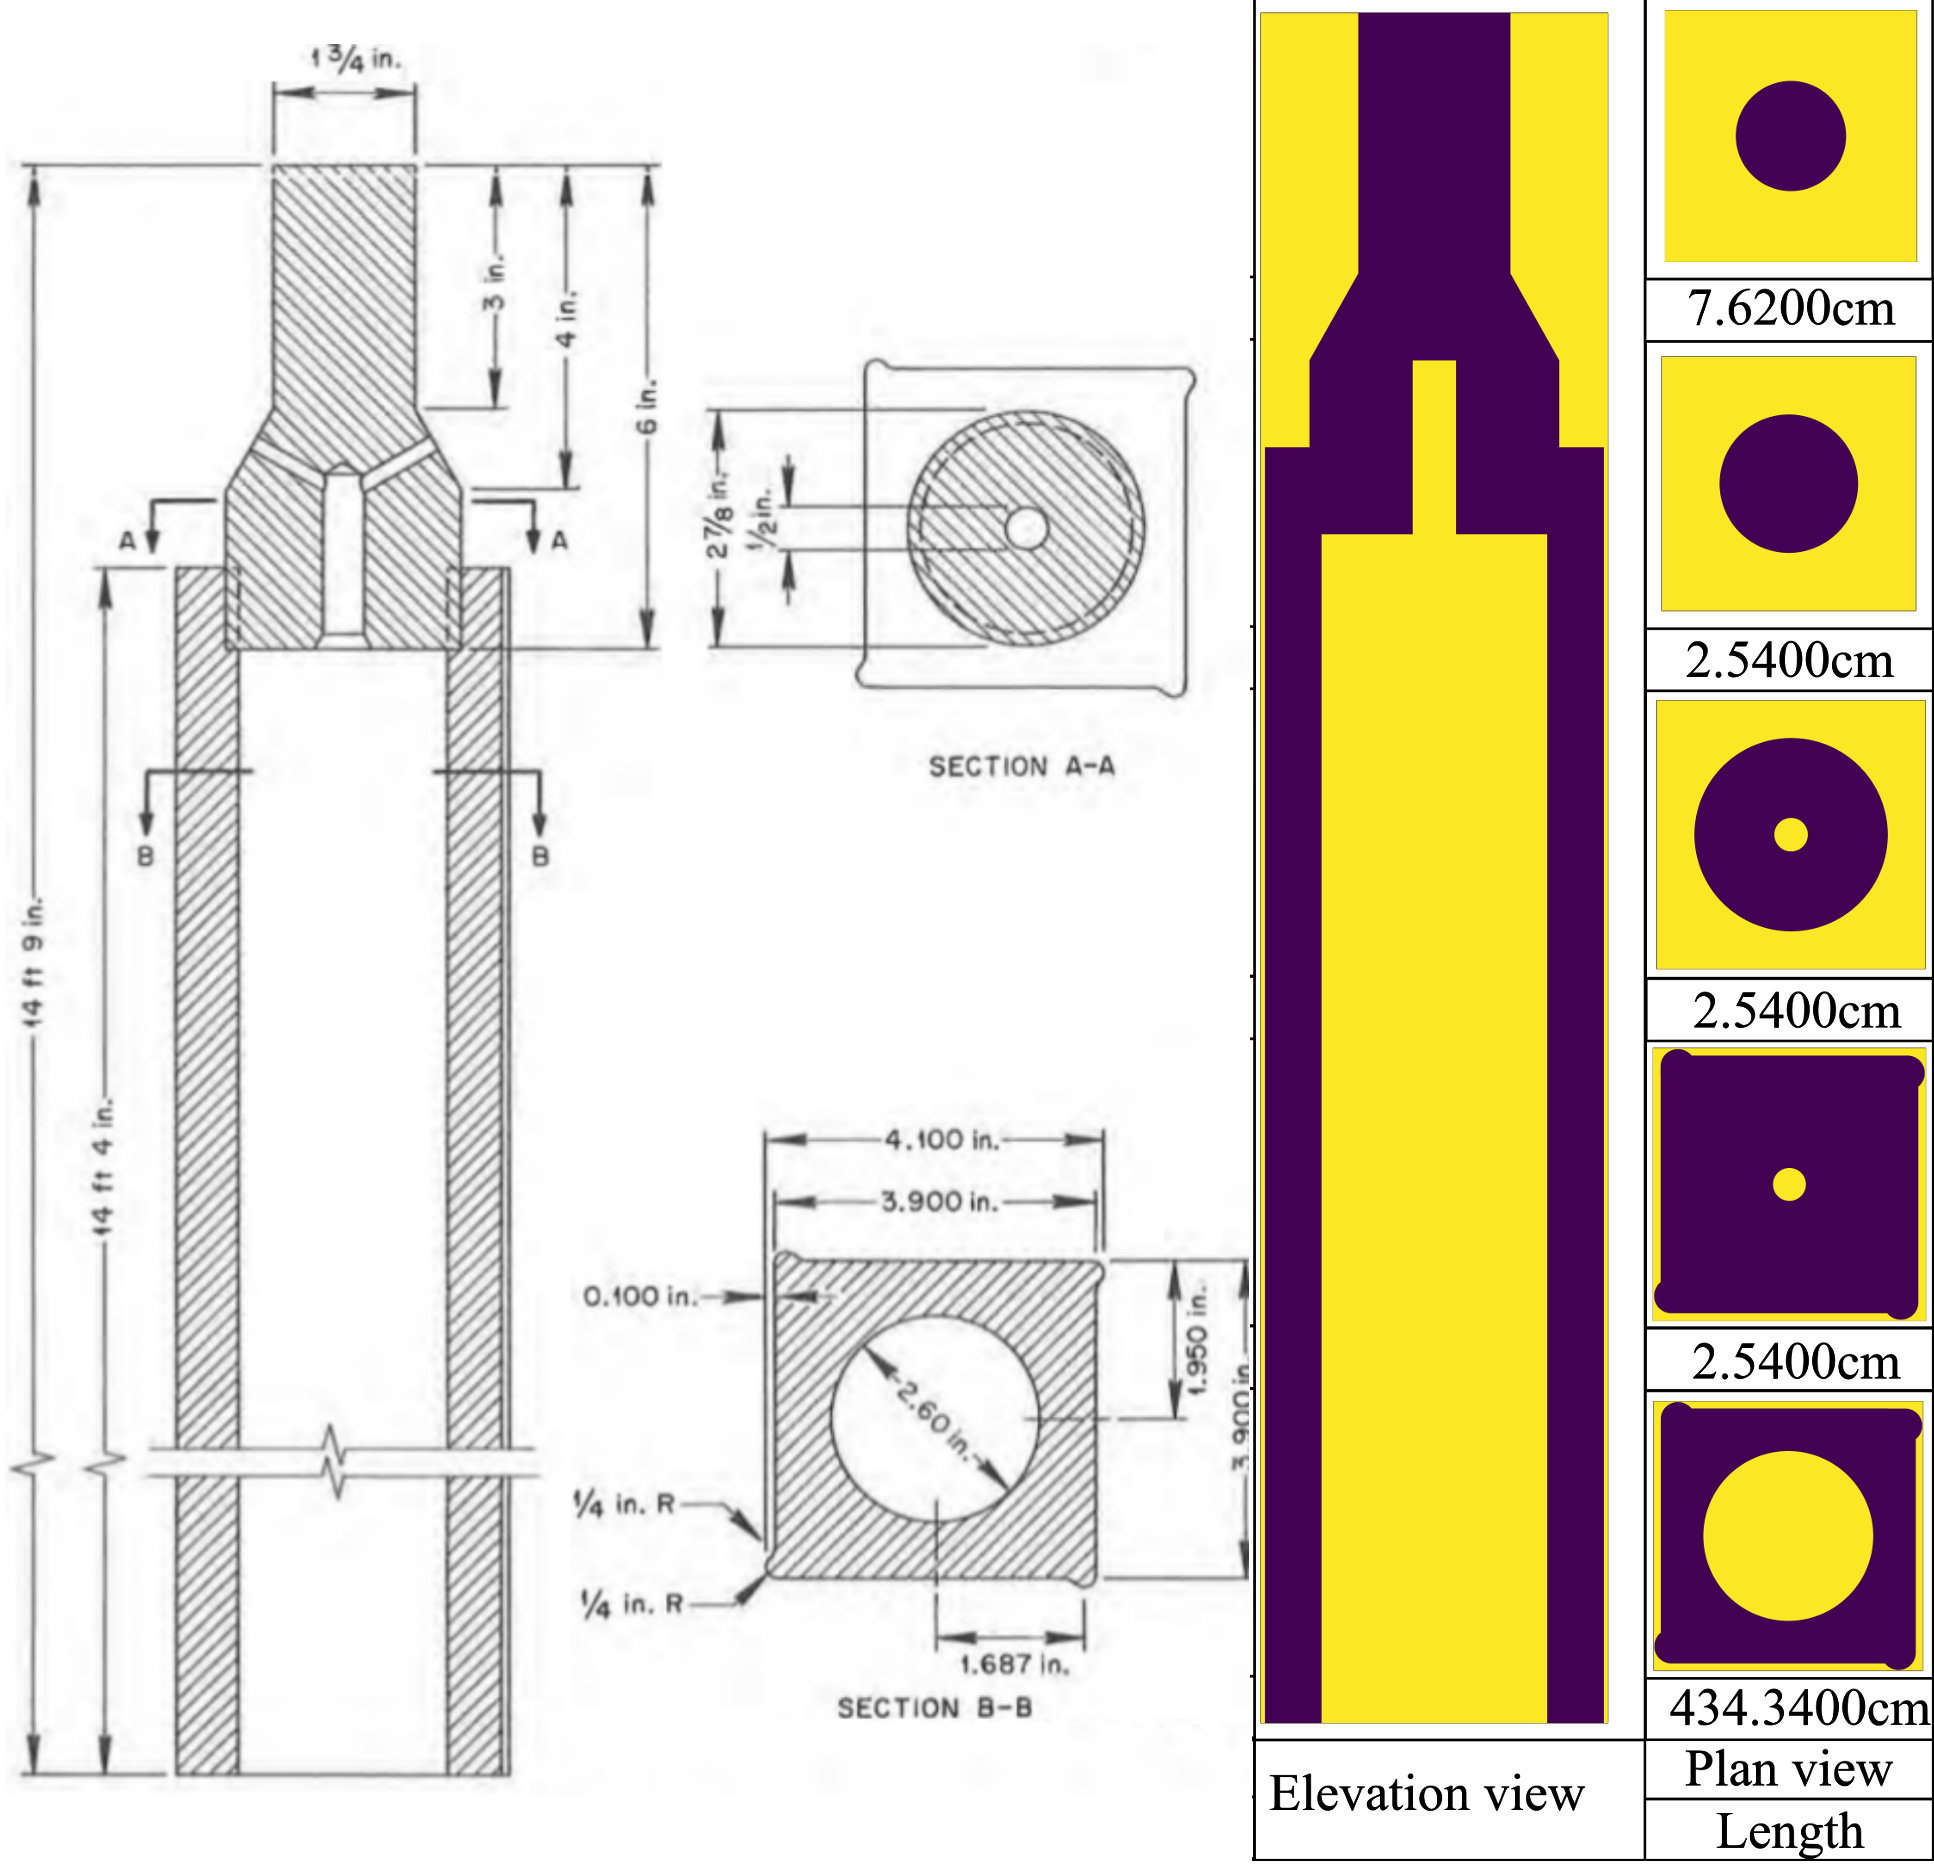
\includegraphics[width=\textwidth]{zone_II_element_ref.png}
  \caption{Graphite moderator elements for zone II-A \cite{robertson_conceptual_1971,rykhlevskii_full-core_2017}.}
  \vspace{-0.6em}
  \label{fig:II_element_ref}
\end{figure}
\FloatBarrier

\section{Existing full-core MSBR models}
There are few recent studies presenting full-core \gls{MSBR} models for neutronics analysis. Park \emph{et al.} developed an MCNP6 model for burnup computations and safety parameter analysis \cite{park_whole_2015}. This model has significant geometry simplifications in zone II-B graphite elements, and entirely neglects lengthwise ridges at each cell corner. Figure~\ref{fig:park} shows the simplifications in the model geometry.  More recently, Skirpan \emph{et al.} built a model of the core using Shift \cite{pandya_implementation_2016} to compare the fidelity of one-cell, two-cell and full-core models of the \gls{MSBR} \cite{skirpan_fuel_2017}. In this model, complex cell geometry in zone I and zone II-A were approximated to slightly rotated square cylinders (figure~\ref{fig:skirpan_cell}). Moreover, as can be seen from figure~\ref{fig:skirpan_plan}, zone II-B was described by Skirpan \cite{skirpan_fuel_2017} using horizontal, vertical and 45$^\circ$-degree graphite elements. These approximations distort neutron flux and reacton rates in that region, and, consequently, may misrepresent breeding parameters of the reactor.

Therefore, full-core Monte Carlo model with sufficient fidelity is necessary for online reprocessing and refueling simulation. Moreover, a high-fidelity model is essential for problem-oriented homogenized nuclear data (multi-group cross sections and diffusion constants) generation for deterministic reactor codes, and for coupled simulations.

\begin{figure}[hbp!] % replace 't' with 'b' to 
  \centering
  \vspace{-0.3em}
  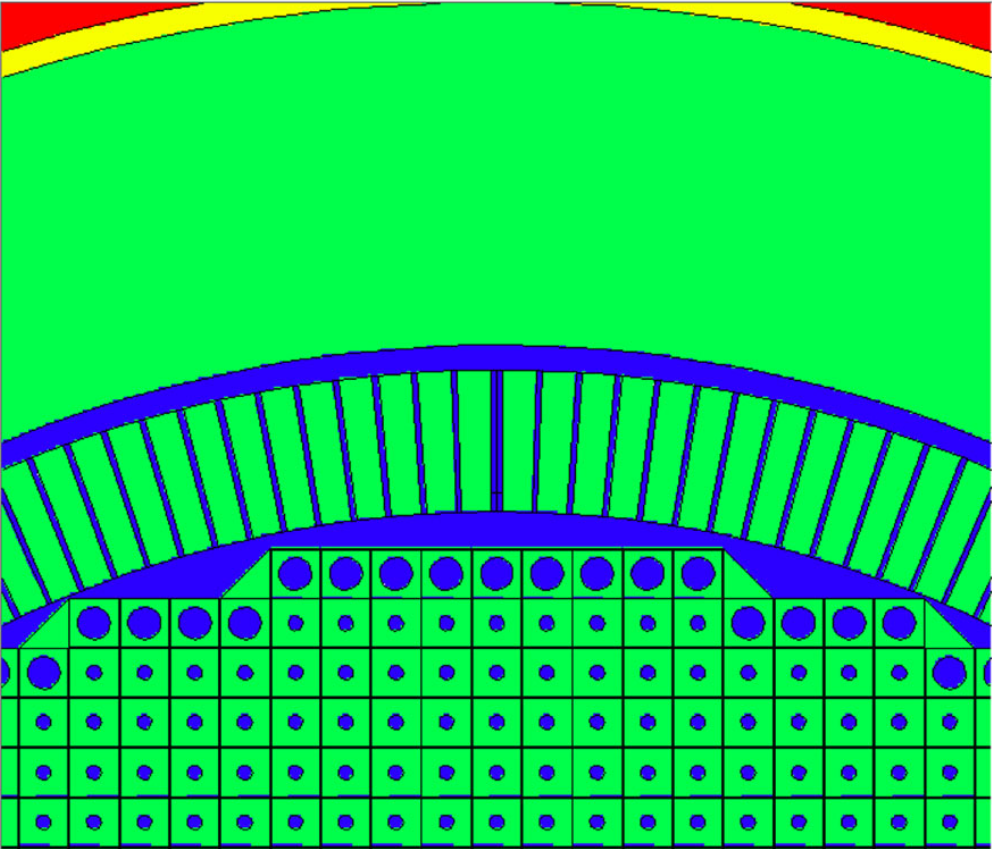
\includegraphics[width=\textwidth]{park_detailed_view.png}
  \caption{Graphite moderator elements  for zone II and reflector from Park \gls{MSBR} model (MCNP6) \cite{park_whole_2015}.}
  \vspace{-0.6em}
  \label{fig:park}
\end{figure}
\FloatBarrier

\begin{figure}[htp!] % replace 't' with 'b' to 
  \centering
  \vspace{-0.3em}
  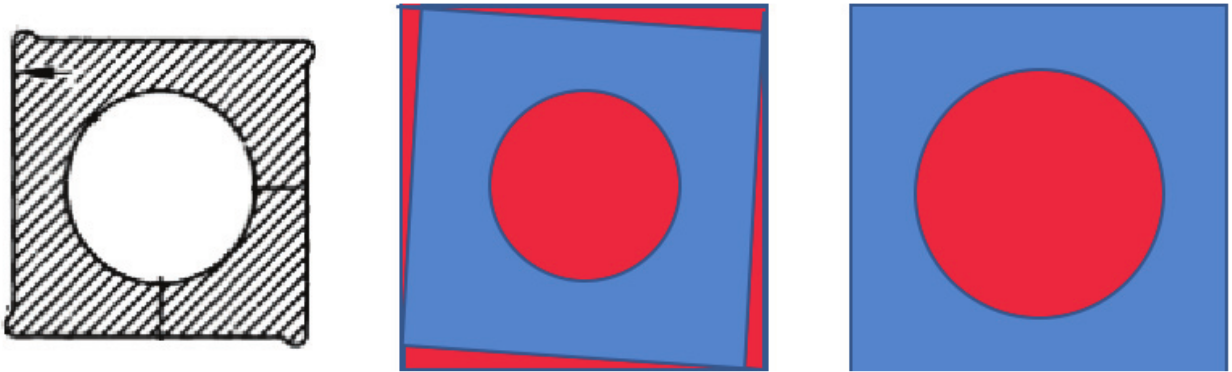
\includegraphics[width=0.95\textwidth]{skirpan_cell.png}
  \caption{Geometry of an MSBR fuel channel (left) approximated with a simple geometric model (center) to calculate appropriate volumes to reduce to a two-region model (right) from Skirpan model (Shift). Red is fuel salt, blue is graphite \cite{skirpan_fuel_2017}.}
  \vspace{-0.6em}
  \label{fig:skirpan_cell}
\end{figure}

\begin{figure}[hbp!] % replace 't' with 'b' to 
  \centering
  \vspace{-0.3em}
  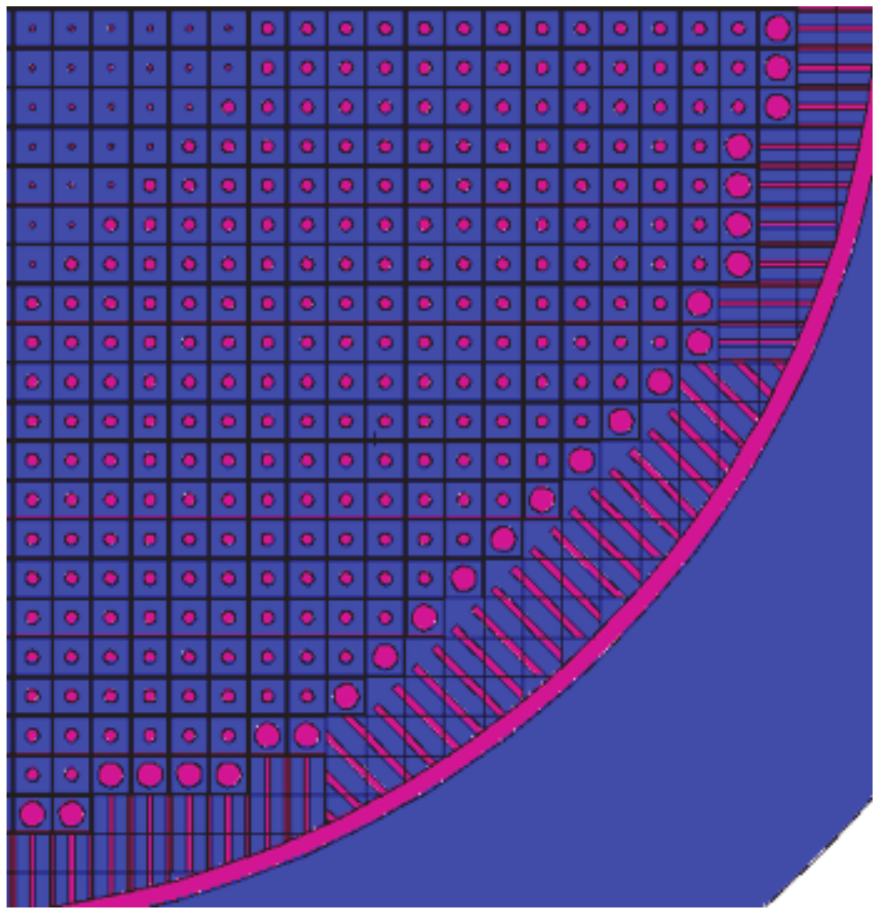
\includegraphics[width=0.7\textwidth]{skirpan_plan_view.png}
  \caption{Plan view of the \gls{MSBR} full-core transport model at core horizontal midplane from Skirpan model (Shift). Pink is fuel salt, blue is graphite \cite{skirpan_fuel_2017}.}
  \vspace{-0.6em}
  \label{fig:skirpan_plan}
\end{figure}
\FloatBarrier

\section{SERPENT 2 model}

Advanced geometry surfaces in SERPENT are employed to represent complex irregular \gls{MSBR} core. Fig.~\ref{fig:serpent_plan_view} shows the plan view of the whole-core configuration at the expected reactor operational level when both graphite control rods are fully inserted, and the safety rods are fully withdrawn. The safety rods only get inserted during an accident and were not inserted in this model. Another feature of the \gls{MSBR}, delayed neutron precursor drift corresponding to its circulating liquid fuel, is not treated here. 

Fig.~\ref{fig:serpent_sectional_view} shows the longitudinal section of the reactor. The violet color represents graphite, and the yellow represents fuel salt. The blue color shows Hastelloy-N, a material used for the plenum and vessel wall, and the white color is a void space. The model contains over 2000 geometric surfaces and 2066 calculation zones. In this thesis, all figures of the core were generated using the built-in SERPENT plotter.

\begin{figure}[hbp!] % replace 't' with 'b' to 
  \centering
  \vspace{-0.3em}
  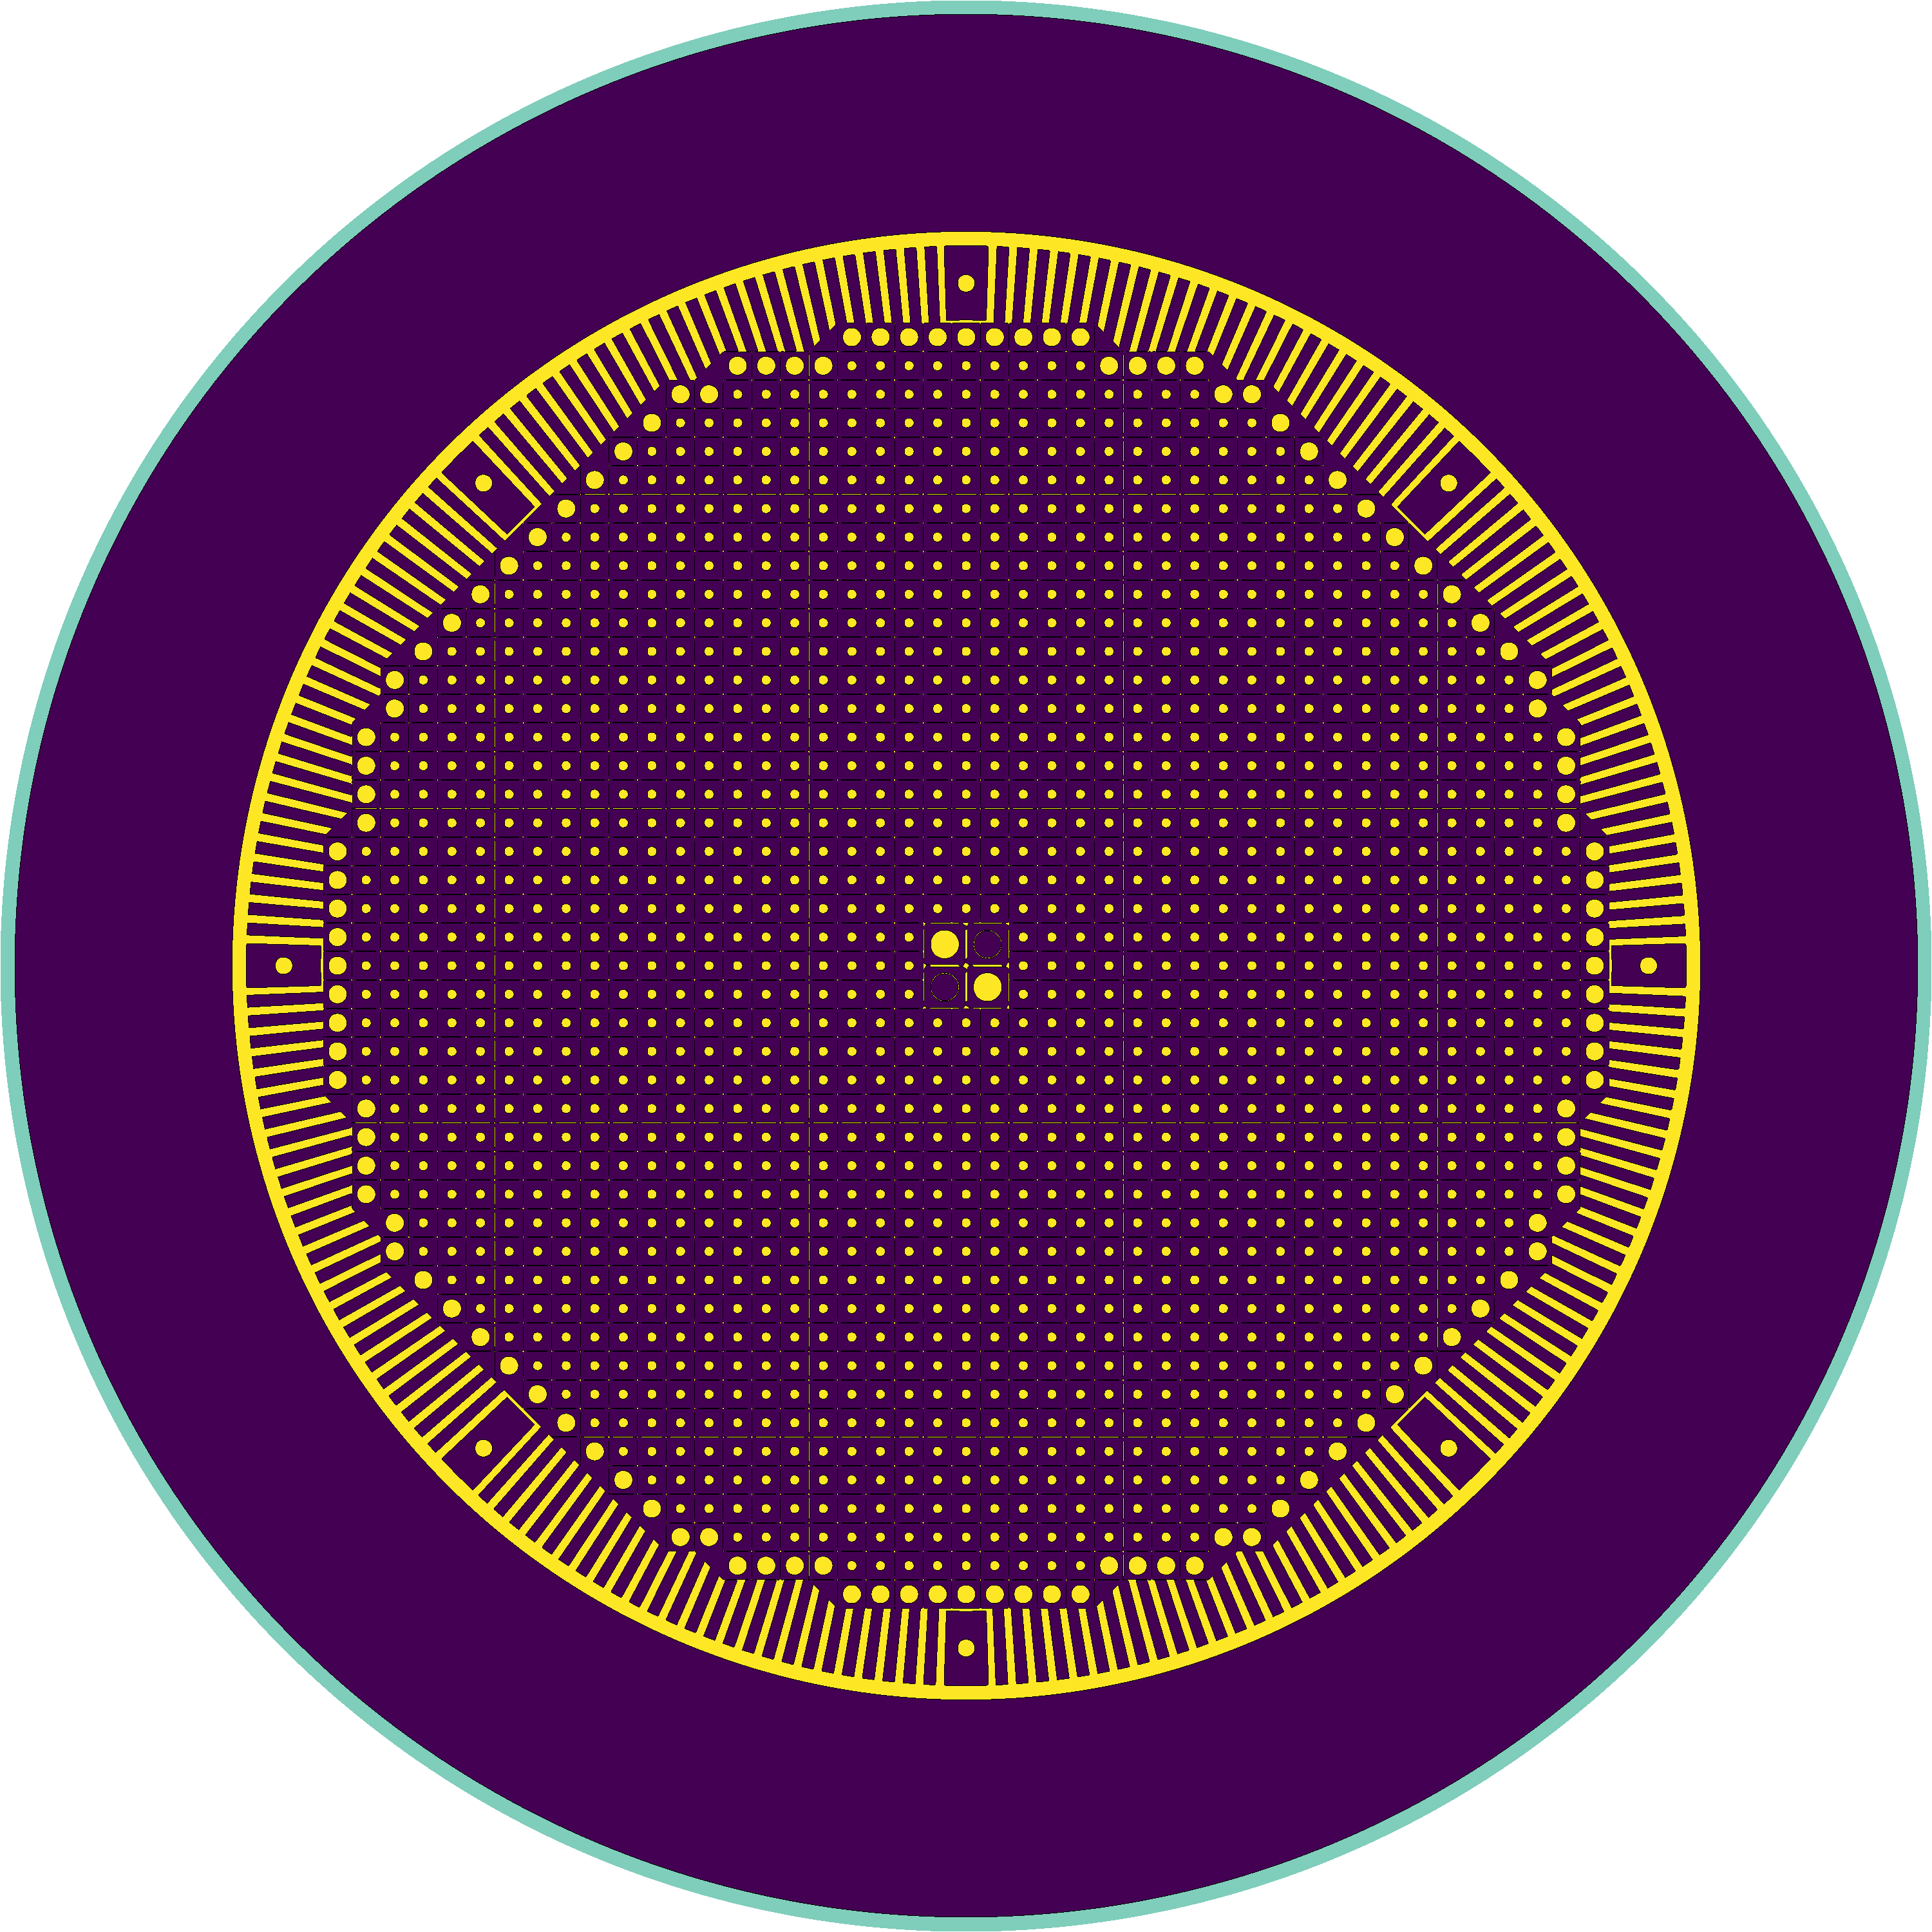
\includegraphics[width=\textwidth]{plan_view_ser.png}
  \caption{Plan view of SERPENT 2 \gls{MSBR} model developed in this work.}
  \vspace{-0.6em}
  \label{fig:serpent_plan_view}
\end{figure}
\FloatBarrier

\begin{figure}[hbp!] % replace 't' with 'b' to 
  \centering
  \vspace{-0.3em}
  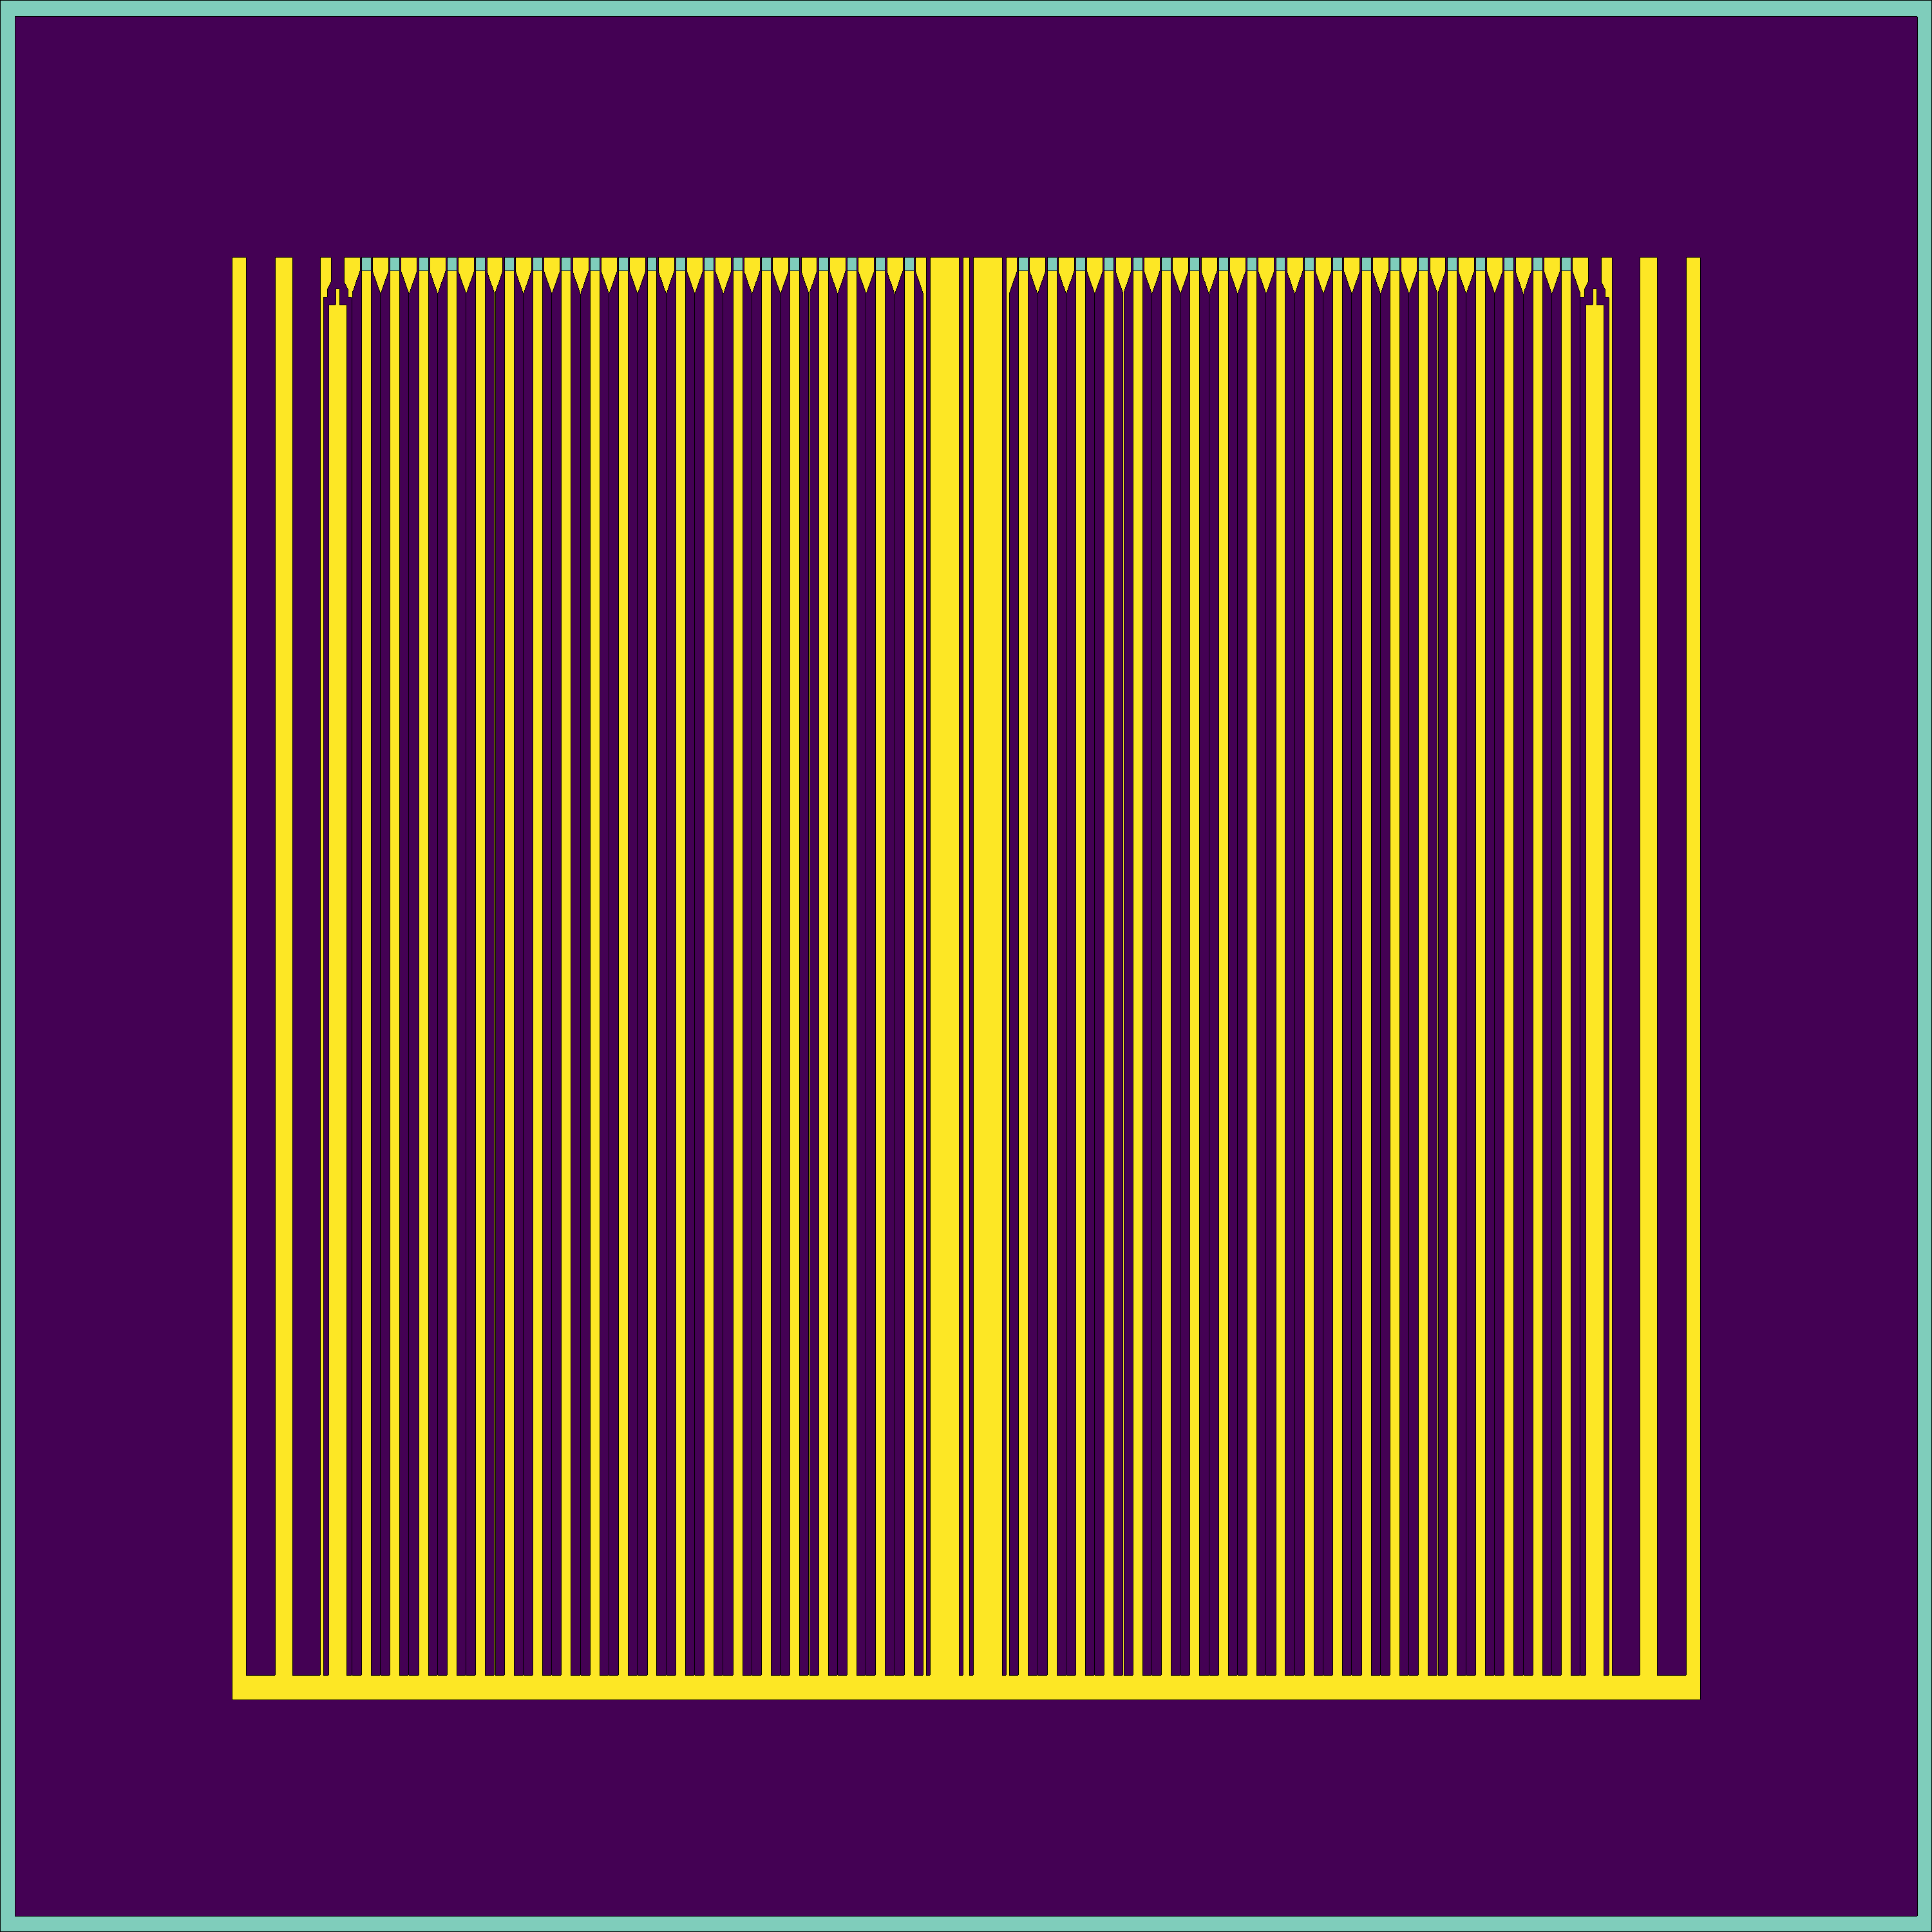
\includegraphics[width=\textwidth]{sect_view_ser.png}
  \caption{Elevation view of SERPENT 2 \gls{MSBR} model developed in this work.}
  \vspace{-0.6em}
  \label{fig:serpent_sectional_view}
\end{figure}
\FloatBarrier

In the model, zone I, zone II-A graphite blocks were described using circular cylinder and square cylinder surface types. The lengthwise ridges at each corner mentioned earlier were specified using dodecagonal cylindrical surfaces and general planes (figure~\ref{fig:I_element_ref}, \ref{fig:II_element_ref}). Zone I of the core was described using square lattices inscribed in the octagonal cylindrical surfaces to accurately represent geometry of that region.

The main challenge was to accurately represent zone II-B because it has irregular elements with sophisticated shapes. From the \gls{ORNL} report \cite{robertson_conceptual_1971}, the suggested design of zone II-B has 8 irregularly-shaped graphite elements every 45$^\circ$ as well as salt channels (figure~\ref{fig:detail_plan_view}). These graphite elements were simplified into right-circular cylindrical shapes  with central channels. Fig.~\ref{fig:serpent_zoneII} illustrates this core region in the SERPENT model. The volume of fuel salt in zone II was kept exactly 37\%, so that this simplification did not considerably change the core neutronics. This is the only simplification made to the \gls{MSBR} geometry in this work. 

\begin{figure}[hbp!] % replace 't' with 'b' to 
  \centering
  \vspace{-0.3em}
  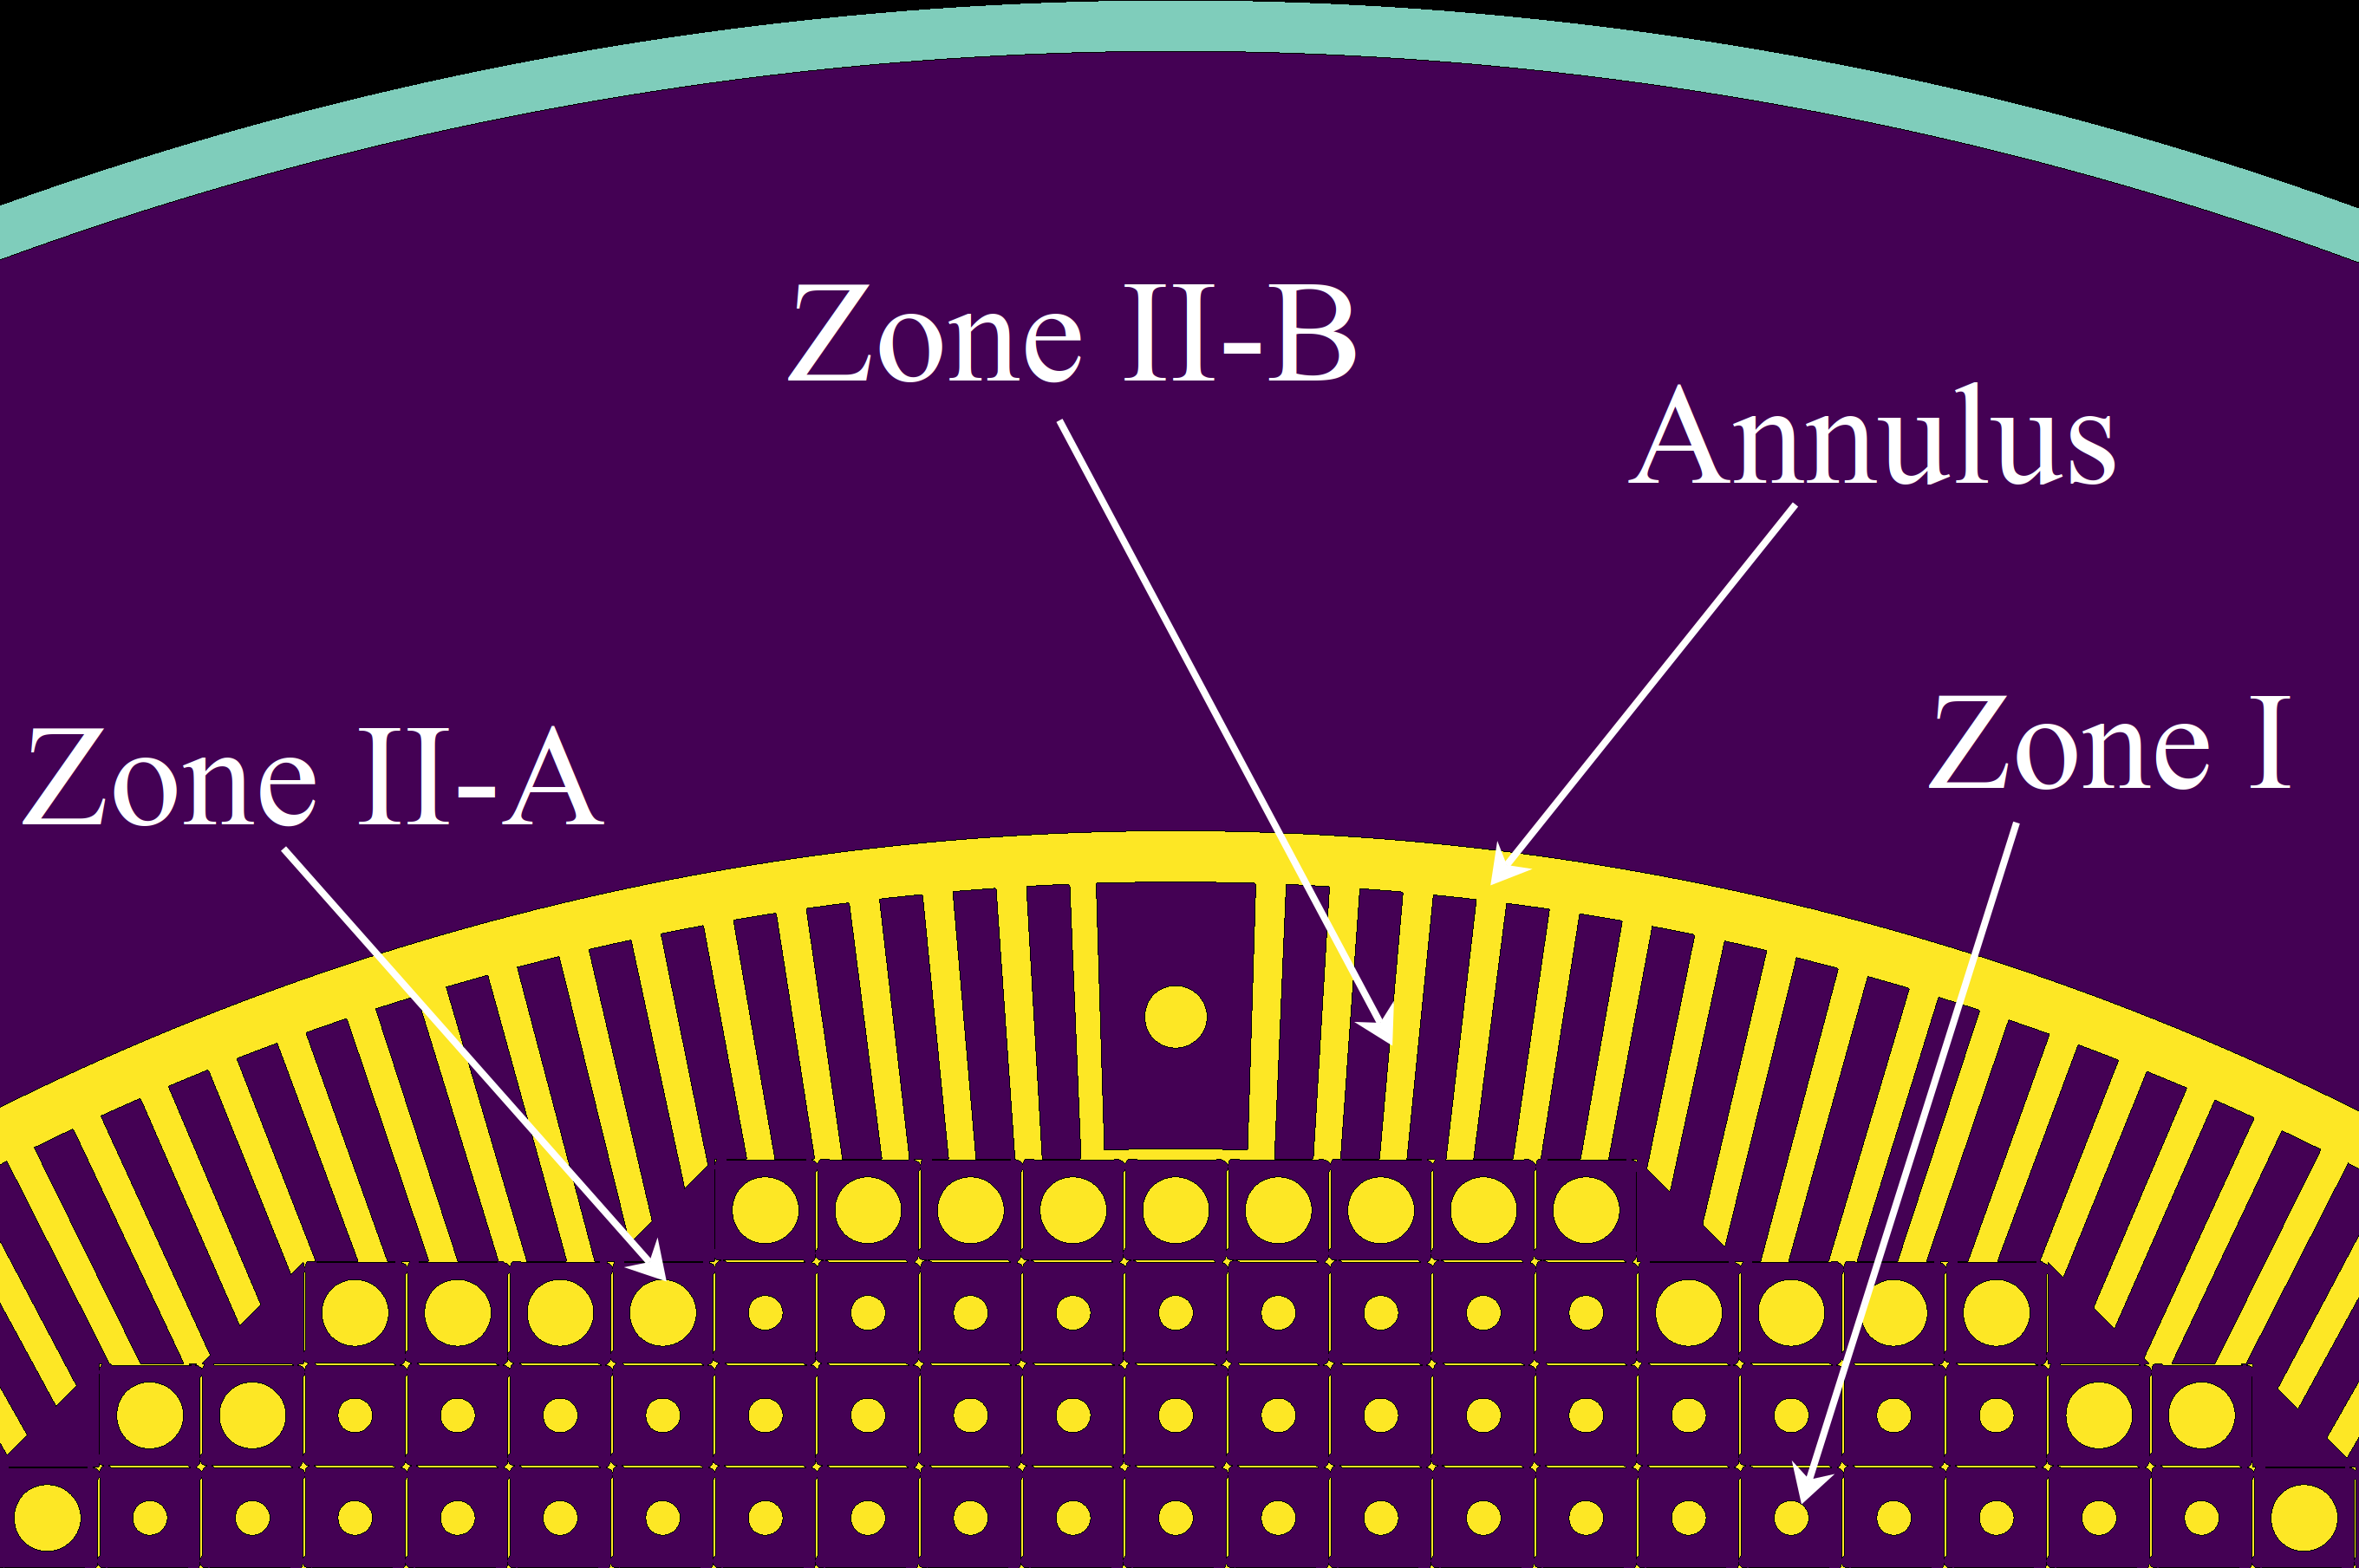
\includegraphics[width=\textwidth]{ser_zone_II.png}
  \caption{Detailed view of \gls{MSBR} zone II model.}
  \vspace{-0.6em}
  \label{fig:serpent_zoneII}
\end{figure}
\FloatBarrier

\subsection{Material composition and normalization parameters}
The fuel salt, the reactor graphite, and the modified Hastelloy-N\footnote{ Hastelloy-N is very common in reactors now but have been studied and developed at \gls{ORNL} in a program that started in 1950s.} are materials unique of the \gls{MSBR} and were created at \gls{ORNL}. The initial fuel salt used the same density (3.35 g/cm$^3$) and composition LiF-BeF$_2$-ThF$_4$-$^{233}$UF$_4$ (71.8-16-12-0.2 mole \%) as the \gls{MSBR} design\cite{robertson_conceptual_1971}. The lithium in the molten salt fuel is fully enriched in $^{7}$Li because $^{6}$Li is a very strong neutron poison and becomes tritium upon neutron capture. 

For cross section generation, JEFF-3.1.2 neutron library was employed \cite{oecd/nea_data_bank_jeff-3.1.2_2014}. The specific temperature was fixed for each material to correctly model the Doppler-broadening of resonance peaks when SERPENT generates the problem-dependent nuclear data library. The isotopic composition of each material at the initial state was described in detail in the MSBR conceptual design study \cite{robertson_conceptual_1971} and has been applied to SERPENT model without any modification. Table~\ref{tab:msbr_tab} is a summary of the major \gls{MSBR} parameters used by this model \cite{robertson_conceptual_1971}. 

%%%%%%%%%%%%%%%%%%%%%%%%%%%%%%%%%%%%%%%%
\begin{table}[h!]
        %\centering
        \caption{Summary of principal data for MSBR \cite{robertson_conceptual_1971}.}
        \begin{tabular}{|m{0.56\linewidth} | m{0.36\linewidth}|}
        \hline
        %\begin{tabularx}{\linewidth}{l X} \toprule 
                Thermal capacity of reactor           & 2250 MW(t)
                \\ [5pt] \hline 
                Net electrical output                 & 1000 MW(e) 
                \\ [5pt] \hline 
                Net thermal efficiency        & 44.4\%
                \\ [5pt] \hline 
                Salt volume fraction in central core zone     & 0.13
                \\ [5pt] \hline 
                Salt volume fraction in outer core zone       & 0.37
                \\ [5pt] \hline 
                Fuel salt inventory (Zone I)                  & 8.2 m$^3$	
                \\ [5pt] \hline 
                Fuel salt inventory (Zone II)                 & 10.8 m$^3$	
                \\ [5pt] \hline 
                Fuel salt inventory (annulus)                 & 3.8 m$^3$	
                \\ [5pt] \hline 
                Total fuel salt inventory                     & 48.7 m$^3$	
                \\ [5pt] \hline 
                Fissile mass in fuel salt                   & 1303.7 kg	
                \\ [5pt] \hline 
                Fuel salt components                  & 
                LiF-BeF$_2$-ThF$_4$-$^{233}$UF$_4$	
                \\ [5pt] \hline 
                Fuel salt composition                 & 
                71.85-16-12-0.25 mole\%
                \\[5pt]  \hline 
                Fuel salt density                    & 
                3.35 g/cm$^3$
                \\[5pt]  \hline 
        \end{tabular}
        \label{tab:msbr_tab}
\end{table}
%%%%%%%%%%%%%%%%%%%%%%%%%%%%%%%%%%%%%%%%%%%%%%%%

